\section{Linear Basis-Functions} \label{cha:Linear_Basis_Function} 
Our first choice of \glspl{basisFunction} are linear polynomials with \gls{localSupport}.
This results in a \gls{FEMSol} supporting \glsentryname{order0Cont}. To span the space of first degree polynomials over an \gls{element}
we need two linearly independent first degree functions. A first degree polynomial needs furthermore two parameters to be fully
specified. We say then a linear polynomial has two degrees of freedom.

\begin{equation} \label{eqn:A_Linear_Polynomial}
	\psi = \psi \left( x \right) = c_0 + c_1 x.
\end{equation}
A \gls{basisFunction} over a single \gls{element} is called a \gls{shapeFunction}. We may use
the two parameters in \cref{eqn:A_Linear_Polynomial} to impose certain values on both end points of the \glspl{shapeFunction}.
Denoting these functions by $\psi_{1}$ and $\psi _{2}$ we may formulate conditions in the \gls{localCoord} as
\begin{subequations} \label{eqn:Cond_On_Linear_Psi_Local}
	\begin{align}
		\psi_{1}\left( 0 \right) & = 1, \label{eqn:Cond_On_Linear_Psi_1_At_Start} \\
		\psi_{1}\left( 1 \right) & = 0, \label{eqn:Cond_On_Linear_Psi_1_At_End} 	\\
		\psi_{2}\left( 0 \right) & = 0, \label{eqn:Cond_On_Linear_Psi_2_At_Start} \\
		\psi_{2}\left( 1 \right) & = 1. \label{eqn:Cond_On_Linear_Psi_2_At_End}
	\end{align}
\end{subequations}
Next we insert conditions in \crefrange{eqn:Cond_On_Linear_Psi_1_At_Start}{eqn:Cond_On_Linear_Psi_2_At_End}
into \cref{eqn:A_Linear_Polynomial}. For each \gls{shapeFunction} we then get two equations with two unknowns, $c_0$ and $c_1$.
Solving these systems give fully specified \glspl{shapeFunction} as 
\begin{subequations}	\label{eqn:Linear_Psi_Local}
	\begin{align}
		\psi_{1} \left( x \right) &= 1 - x, \\
		\psi_{2} \left( x \right) &= x.
	\end{align}
\end{subequations}
\begin{figure}
	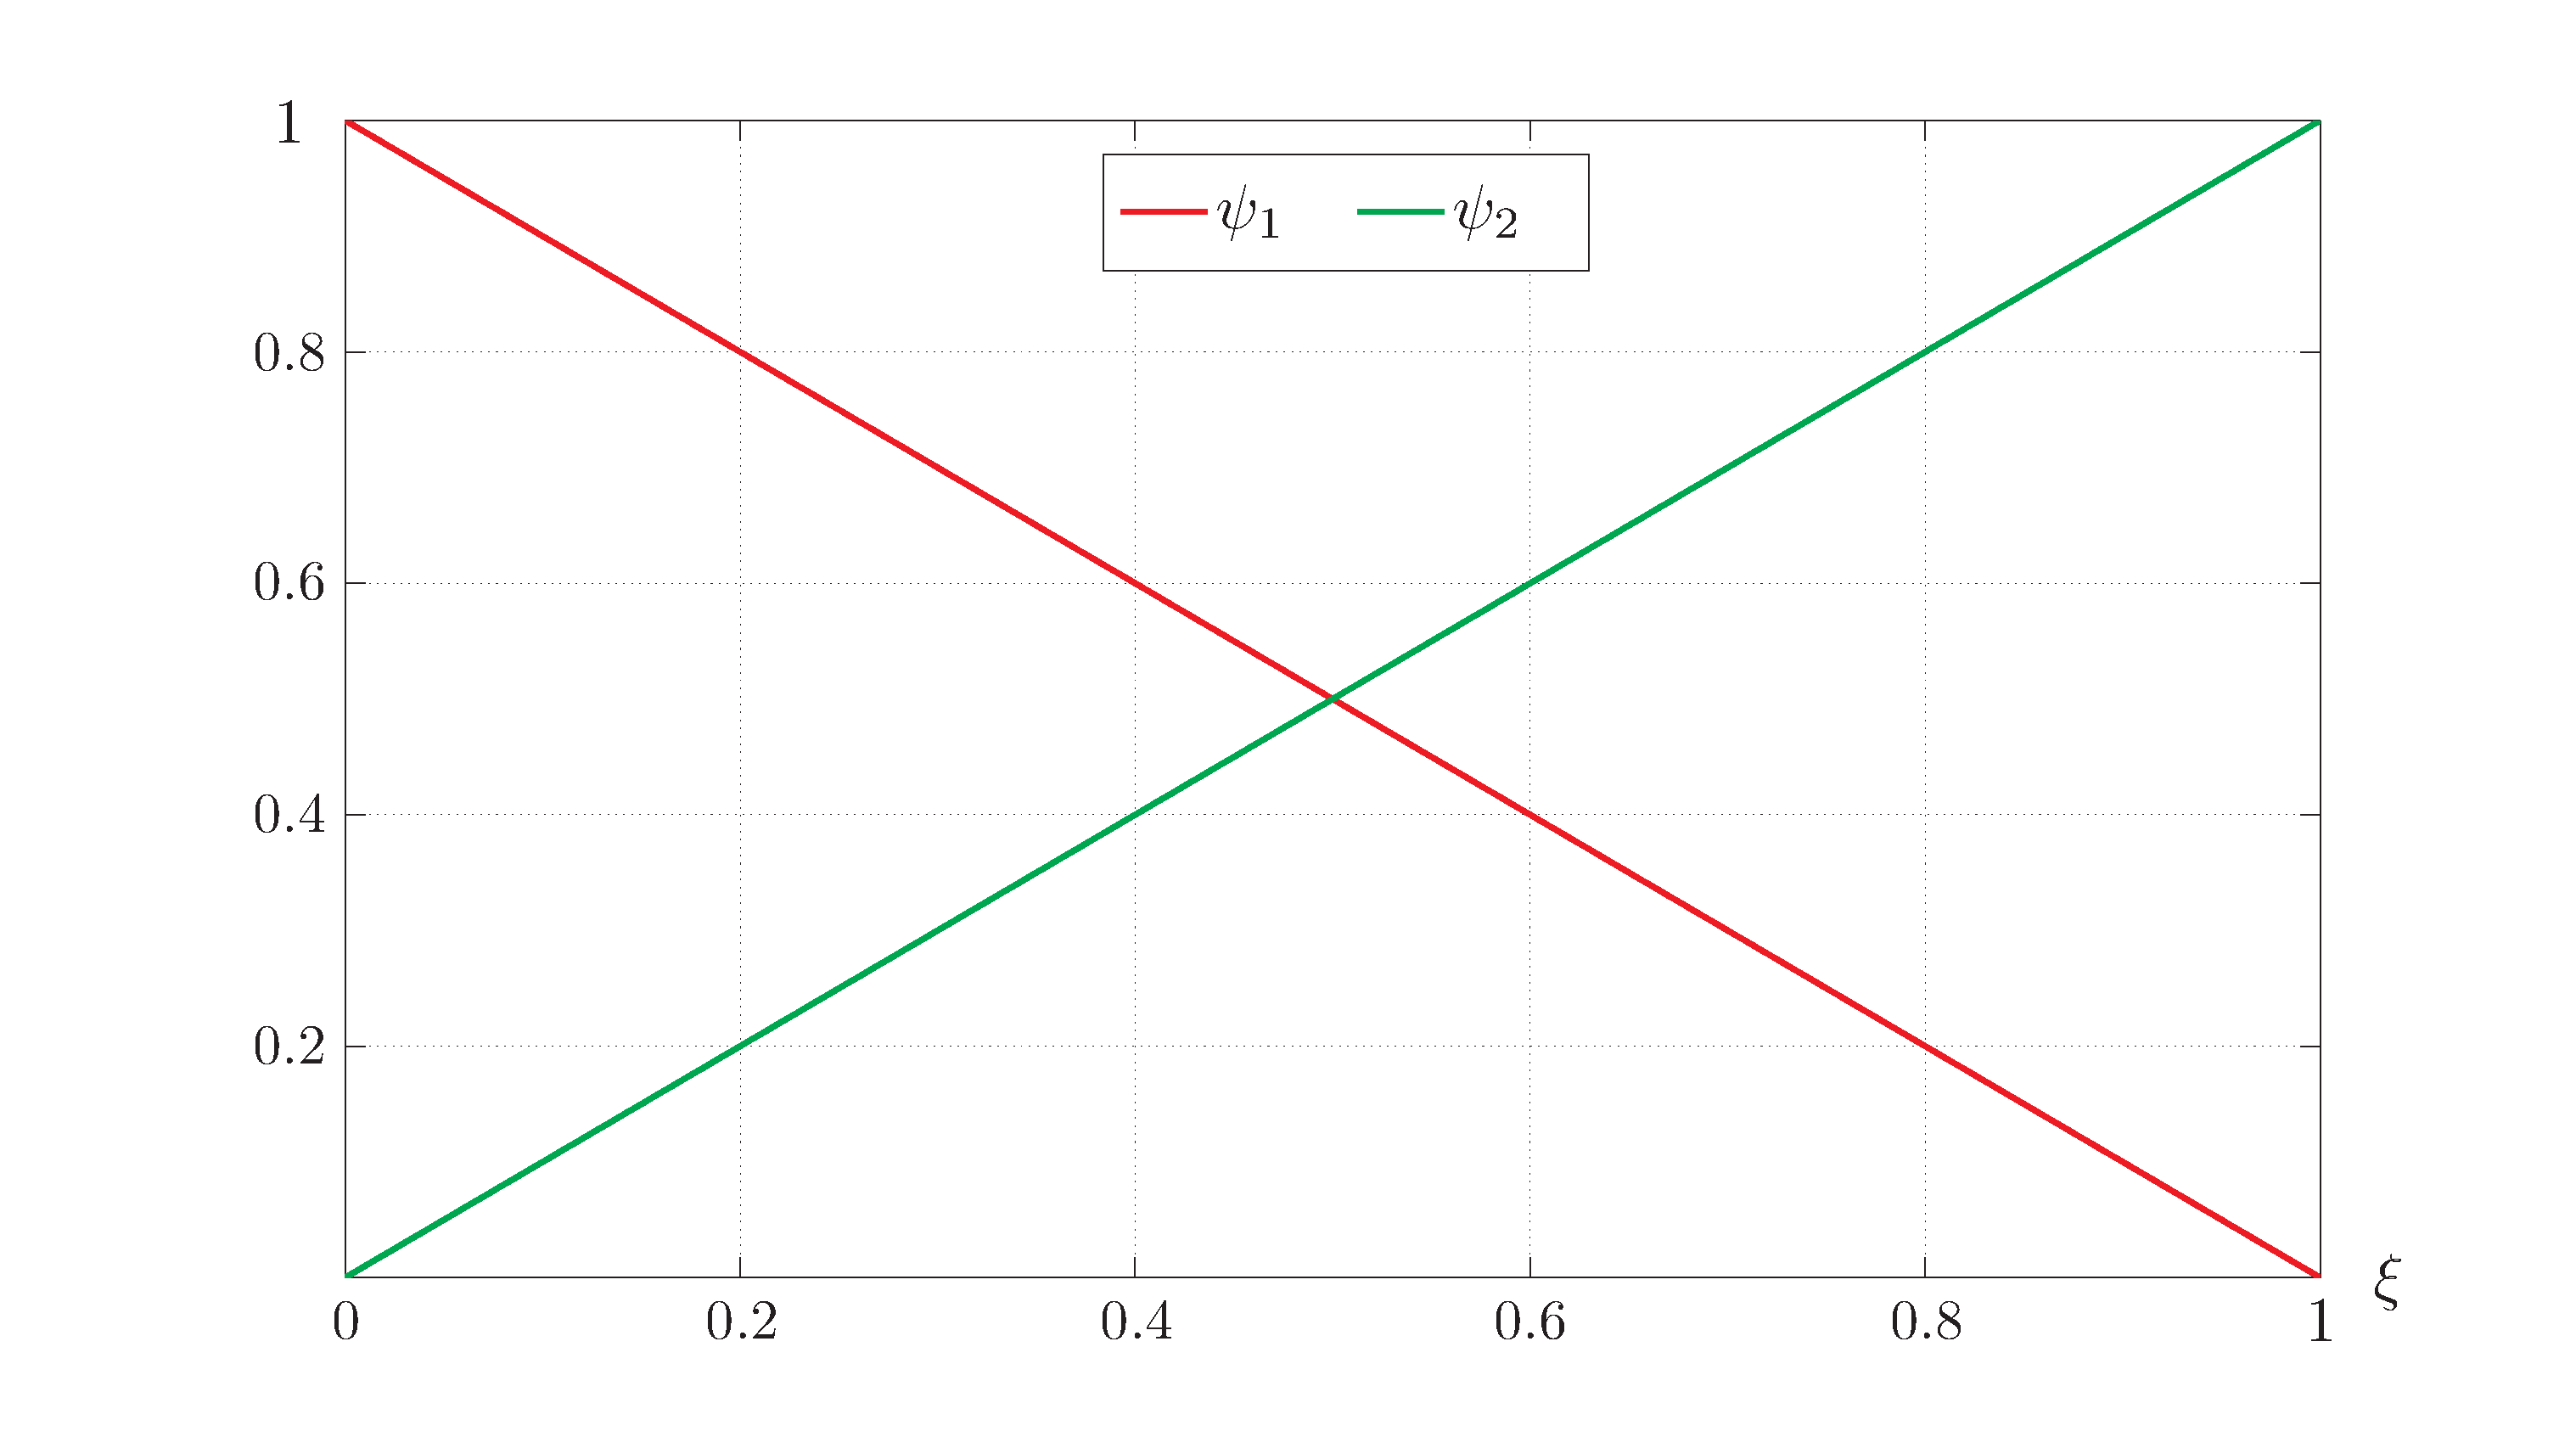
\includegraphics[width = \textwidth]{../figures/linear-shape-functions}
	\caption[Choice of Linear Polynomials for Shape Functions]{Choice of Linear Polynomials for Shape Functions}
	\label{fig:Linear_Shape_Functions}
\end{figure}
\begin{figure}
	
\includegraphics[width = \textwidth]{../Figures/linear-basis-functions}
	\caption[Choice of Cubic Polynomials for Basis-Functions]
		{Choice of linear polynomials for Basis-Functions gives a solution which is $\mathcal{O} \left( 0 \right)$-continuous.}
		\label{fig:Linear_Basis_Functions}
\end{figure}
The linear \glspl{shapeFunction} and \gls{piecewiseLinear} polynomials over the whole \gls{region} are shown in
\cref{fig:Linear_Shape_Functions,fig:Linear_Basis_Functions}, respectively. Observe that a \gls{basisFunction} $\varphi _{i}\left( x\right)$
consists of two \glspl{shapeFunction} joined at \gls{nodePoint} $x_{i}$. \Glspl{basisFunction} are therefore \gls{piecewiseLinear} polynomials.
We see clearly that \glspl{basisFunction} support \glsentryname{order0Cont}. Thus for $i = 2, 3, \dots, N$
\begin{subequations} \label{eqn:Phi_i_Linear}
	\begin{align}
		\varphi_{i} \left( x_{i-1} \right) & = 0,  \label{eqn:Phi_i_At_Left_End} \\
		\lim_{x \rightarrow x_{i}^{-}} \varphi_{i} \left( x \right) & =
		\lim_{x \rightarrow x_{i}^{+}} \varphi_{i} \left( x \right) = 1,	\label{eqn:Phi_i_At_Center} \\
		\varphi_{i}\left( x_{i + 1} \right) & = 0.  \label{eqn:Phi_i_At_Right_End}
	\end{align}
\end{subequations}
Conjuncture is irrelevant for the first and last \glspl{basisFunction}, due to the fact that they are only defined over one element. Thus
\begin{subequations} \label{eqn:Phi_Boundaries}
	\begin{align}
		\varphi_{1} \left( x_{1} \right) & = 1,  \label{eqn:Phi_1_At_x_1} \\
		\varphi_{1} \left( x_{2} \right) & = 0,  \label{eqn:Phi_1_At_x_2} \\
		\varphi_{N + 1} \left( x_{N} \right) & = 0,  \label{eqn:Phi_N_Plus_1_At_x_N} \\
		\varphi_{N + 1} \left( x_{N + 1} \right) & = 1.  \label{eqn:Phi_N_Plus_1_At_x_N_Plus_1}
	\end{align}
\end{subequations}
\Gls{nodePoint} $x_{i}$ where $\varphi _{i}$ takes on the unity value is called the home node of $\varphi _{i}$. The node point
$x_{i}$ is also the joint point between two pieces of linear polynomials and thus the condition in \cref{eqn:Phi_i_At_Center}
guarantees \glsentryname{order0Cont}. Furthermore, for $j = 1, 2, \dots, N$, \cref{eqn:Phi_i_Linear} results in
\begin{equation} \label{eqn:u_At_x_j}
	\begin{aligned}
		\glsentryname{uAtXj} & = \sum_{i = 1}^{N + 1} \glsentryname{ai} \glsname{phii} \Big \vert_{x = x_j} \\
		& = a_j \varphi_{j} \left( x_j \right) \\
		& = a_j.
	\end{aligned}
\end{equation}
As we see later we can use \cref{eqn:u_At_x_j} to implement the Dirichlet condition on the left boundary.
%
\subsection[Element Matrix]{\Gls{elementMatrix}} \label{cha:Element_Matrix_Linear}
The global integral involved in calculation of the \gls{stiffnessMatrix} in \cref{eqn:Stiffness_Matrix} may be written as a sum of
integrals each over a single \gls{element}, i.e., 
\begin{equation} \label{eqn:Stiffness_Entries_Linear_1}
	\begin{aligned}
			\glsentryname{Kij} &= \int_{x = 0}^{1} \gls{q} \glsentryname{phiiPrime} \glsentryname{phijPrime} \dd x \\
			&= \sum \limits_{e = 1}^{\gls{N}} \int_{x \in \Omega_{e}} \gls{q} \glsentryname{phiiPrime} \glsentryname{phijPrime} \dd x.
	\end{aligned}
\end{equation}
Observe that $\varphi_i \left( x \right)$ is only non-zero over the two \gls{adjacentElements} $\Omega_{i - 1}$ and $\Omega_{i}$.
In the same manner $\varphi_j \left( x \right)$ is only non-zero over $\Omega_{j - 1}$ and $\Omega_{j}$. Thus the global stiffness
matrix is tridiagonal, i.e.,
\begin{equation}	\label{eqn:Global_Stiffness_Properties}
	\begin{aligned}
			\gls{Kij}	&= K_{j,i} \neq 0, 	&&	j = i - 1,  i,  i + 1, \\
			\gls{Kij}	&= K_{j,i} = 0, 	&&	\text{otherwise.}
	\end{aligned}
\end{equation}
\Cref{eqn:Stiffness_Entries_Linear_1} is then reduced to
\begin{subequations}	\label{eqn:Stiffness_Linear}
	\begin{align}
		\glsentryname{Kij} &= \int_{ x_{i - 1} }^{ x_{i} } \gls{q} \glsentryname{phiiPrime} \glsentryname{phijPrime} \dd x
		+\int_{ x_{i} }^{ x_{i + 1} } \gls{q} \glsentryname{phiiPrime} \glsentryname{phijPrime} \dd x.
		\label{eqn:Stiffness_Entries_Linear}
	\end{align}
	Thus
	\begin{align}
		K_{i, i} &= \int_{ x_{i - 1} }^{ x_{i} } \gls{q} \bigg( \glsentryname{phiiPrime} \bigg)^2 \dd x
				+\int_{ x_{i} }^{ x_{i + 1} } \gls{q} \bigg( \glsentryname{phiiPrime} \bigg)^2 \dd x
			\label{eqn:Stiffness_Linear_Diag0_1} \\
		K_{i, i + 1} &= K_{i + 1, i} = \int_{ x_{i} }^{ x_{i + 1} } \gls{q} \frac{ d \varphi_i }{ dx } \frac{ d \varphi_{i + 1} }{ dx } \dd x.
			\label{eqn:Stiffness_Linear_Diag1_1}
	\end{align}
\end{subequations}
Consider now \cref{eqn:Stiffness_Linear_Diag1_1} and note that it consists of contribution from a single element,
$\Omega_{i}$. We have derived shape functions in terms of the local variable $\xi \in \left[ 0, 1 \right]$. Generally speaking,
we need then a transformation from the global variable $x \in \Omega_{e} = \left[ x_e, x_{e + 1} \right]$ to the local variable
$\xi \in \left[ 0, 1 \right]$. This brings the global basis-function $\varphi_i$ back to the local shape functions
$\psi_m, \quad m = 1, 2$. The variable change is given by
\begin{equation}	\label{eqn:Global_2_Local_1}
	\begin{alignedat}{3}
		\xi	  &= \frac{x-x_{e}}{x_{e+1}-x_{e}}	\quad& \Leftrightarrow \quad&& x  &= x_{e}+\left(x_{e+1}-x_{e} \right) \xi, \\
		d \xi &= \frac{1}{x_{e + 1} - x_{e}} dx	\quad& \Leftrightarrow \quad&& dx &= \left(x_{e+1}-x_{e} \right) d \xi.
	\end{alignedat}
\end{equation}
Assuming a uniform discretization the change of variable is simplified to
\begin{equation}	\label{eqn:Global_2_Local}
	\begin{alignedat}{3}
		\xi		&= 1 - e + \frac{1}{h} \quad& \Leftrightarrow \quad&&	x  &= \left( e - 1 + \xi \right) h,	\\
		d \xi	&= \frac{1}{h} dx \quad& \Leftrightarrow \quad&&		dx &= hd \xi.
	\end{alignedat}
\end{equation}
Now apply the transformation in \cref{eqn:Global_2_Local} with $e = i$ to \cref{eqn:Stiffness_Linear_Diag1_1}. Then
\begin{subequations}
	\begin{align}
		K_{i, i + 1} &= K_{i + 1, i} = \int_{ ih }^{ \left( i + 1 \right) h } \gls{q} \frac{ d \varphi_i }{ dx }
			\frac{ d \varphi_{i + 1} }{ dx } \dd x	\label{eqn:Element_Stiffness_Entries_1} \\
		&= \int_{ 0 }^{ 1 } q \Bigl[ \left( i - 1 + \xi \right) h \Bigr] \frac{ d \psi_1 }{ d \xi } \frac{d \xi}{ dx }
			\frac{ d \psi_2 }{ d \xi } \frac{ d \xi }{dx} \dd \xi.	\label{eqn:Element_Stiffness_Entries_2} 
	\end{align}
\end{subequations}
Note that \cref{eqn:Element_Stiffness_Entries_1} is deduced from \cref{eqn:Element_Stiffness_Entries_2} by applying Chain Rule to 
$\frac{ d \varphi_i }{ dx }$ and $\frac{ d \varphi_{i + 1} }{ dx }$. Some simplification gives
\begin{align}
		K_{i, i + 1} &= K_{i + 1, i} = \frac{1}{h} \int_{0}^{1} q \Bigl[ \left( i - 1 + \xi \right) h \Bigr] \frac{ d \psi_1 }{ d \xi } \frac{ d \psi_2 }{ d \xi } \dd \xi.
\end{align}
Applying variable transformation in \cref{eqn:Global_2_Local} with $e = i - 1$ and $e = i$ to \cref{eqn:Stiffness_Linear_Diag0_1} 
we get
\begin{equation}
	\begin{split}
		K_{i, i} &= \frac{1}{h} \int_{0}^{1} q \Bigl[ \left( i - 2 + \xi \right) h \Bigr]
			\biggl( \frac{ d \psi_1 }{ d \xi } \biggr)^2 \dd \xi	\\
		&\quad + \frac{1}{h} \int_{0}^{1} q \Bigl[ \left( i - 1 + \xi \right) h \Bigr]
			\biggl( \frac{ d \psi_2 }{ d \xi } \biggr)^2 \dd \xi.
	\end{split}
\end{equation}
Calculation of \gls{Kij} is then summarized by
\begin{subequations}
	\begin{equation}
		\begin{aligned}
			\gls{Kij}	&= K_{22}^{i - 1} + K_{11}^{i},	&& j = i,	\\
			\gls{Kij}	&= K_{j,i} = K_{1,2}^i,			&& j = i - 1, i + 1,	\\
			\gls{Kij}	&= 0,							&& otherwise,
		\end{aligned}
	\end{equation}
	where \glsentryname{Kmne} represents contribution of element No. $e$ to the global stiffness matrix given by
	\begin{equation}	\label{eqn:Element_Stiffness_Entries_3}
		\glsentryname{Kmne} = \int_{0}^{1} q \Bigl[ \left( e - 1 + \xi \right) h \Bigr]
			\frac{ d \psi_m }{ d \xi } \frac{ d \psi_n }{ d \xi } \dd \xi,	\quad m, n = 1, 2.
	\end{equation}
\end{subequations}
%
\subsection[Element Load]{\Gls{elementLoad}} \label{cha:Element_Load_Linear}
Summation over all \glspl{element} may also be carried out under calculation of the global \gls{loadVector}. For simplicity we repeat load vector
components from \cref{eqn:Load_Vector}
\begin{equation}
	\glsentryname{bi} = P  \varphi _{i}\left( x \right) \Bigg \vert_{x = 1} +
	\int_{0}^{1} \gls{f} \gls{phii} \dd x.
\end{equation}
Note again that the only non-zero basis-function at $x = 1$ is the last one, i.e.,
\begin{align}
	\varphi_i \left( x \right) \Big \vert_{x = 1} &= 
	\begin{cases}
		0,	& i = 1, 2, \dots, N,	\\
		1,	& i = N + 1.
	\end{cases}
\end{align}
Then load entries are given by
\begin{subequations}	\label{eqn:Linear_Load_Components}
	\begin{align}
		b_{i} &= \int_{0}^{1} \gls{f} \gls{phii} \dd x - \int_{0}^{1} \gls{q} \glsentryname{thetaPrime} \dd x,
			\quad 1 \leq i \leq \gls{N}, \label{eqn:Typical_Load_Component} \\
		b_{N + 1} &= P + \int_{0}^{1} \gls{f} \varphi_{N + 1} \left( x \right) \dd x.	\label{eqn:Last_Load_Component} 
	\end{align}
\end{subequations}
Now applying variable transformation in \cref{eqn:Global_2_Local} to a typical load element in \cref{eqn:Typical_Load_Component} gives
\begin{equation} \label{eqn:Load_Summation}
		\glsentryname{bi}	= h \int_{ 0 }^{ 1 } f \Bigl[ \left( i - 2 + \xi \right) h \Bigr] \psi_2 \left( \xi \right)
			+ h \int_{ 0 }^{ 1 } f \Bigl[ \left( i - 1 + \xi \right) h \Bigr] \psi_1 \left( \xi \right).
\end{equation}
We will look at the first and last entry of load vector shortly. A typical global load element is given by
\begin{subequations}
	\begin{equation}
		b_{i} = b_{2}^{i - 1} + b_{1}^{i},	\quad i = 2, ... N,
	\end{equation}
	where
	\begin{equation}
		\begin{split}
			b_{m}^{e} &= h \int_{ 0 }^{ 1 } f \Bigl[ \left( e - 1 + \xi \right) h \Bigr] \psi_m \left( \xi \right)	\\
			&\quad -h \int_{0}^{1} q \Bigl[ \left(e-1+\xi \right) h \Bigr] \glsentryname{thetaPrime} \dd \xi, \quad m = 1,2.	
		\end{split}
	\end{equation}
\end{subequations}
%
\subsection{Assembly Process} \label{cha:Assembly_Process_Linear}
We have seen how to construct \glspl{elementMatrix} and \glspl{elementLoad}. \emph{\Gls{assembly}}
is a process where we go through all \glspl{element} and add each element's contribution, i.e., \gls{elementMatrix} and
\gls{elementLoad}, to the global \gls{stiffnessMatrix} and \gls{loadVector}. \\

Now, denote by $\gls{K}$ and $\gls{b}$ the global \gls{stiffnessMatrix} and the global \gls{loadVector}.
Furthermore, let \gls{KGlobalE} and \gls{bGlobalE} denote the global \gls{stiffnessMatrix} and the global \gls{loadVector}
after contributions from elements $1, 2, \dots, e$ are added. Thus $\gls{K} = \mathbf{K}^{ \left( N \right) }$ and
$b = \mathbf{b}^{\left( N \right)}$. Then in a \gls{region} with $N = 4$ \glspl{element}, the global
stiffness matrix and load vector is constructed by a stepwise process sketched in
\crefrange{fig:K_1_Linear}{fig:K_4_Linear} and \cref{fig:b_1_To_b_4_Linear}, respectively.
%
% --------------- Insert Visualization of Linear Assembly Process --------------
% Linear K^{1}
\begin{figure}[H]
	\centering
	\begin{equation*}
		\mathbf{K}^{\left( 1 \right)} =
		\begin{bmatrix}
			k_{11}^{1} & k_{12}^{1} & 0 & 0 & 0 \\ \\
			k_{21}^{1} & k_{22}^{1} & 0 & 0 & 0 \\ \\
			0 & 0 & 0 & 0 & 0 \\ \\
			0 & 0 & 0 & 0 & 0 \\ \\
			0 & 0 & 0 & 0 & 0
		\end{bmatrix}
	\end{equation*}
	\caption{Stiffness Assembly with Linear Basis-Functions, $\mathbf{K}^{\left(1\right)}$ }
	\label{fig:K_1_Linear}
\end{figure}
% Linear K^{2}
\begin{figure}[H]
	\centering
	\begin{equation*}
		\mathbf{K}^{\left( 2 \right)} =
		\begin{bmatrix}
			k_{11}^{1} & k_{12}^{1} & 0 & 0 & 0 \\ \\
			k_{21}^{1} & k_{22}^{1} + k_{11}^{2} & k_{12}^{2} & 0 & 0 \\ \\
			0 & k_{21}^{2} & k_{22}^{2}	& 0 & 0 \\ \\
			0 & 0 & 0 & 0 & 0 \\ \\
			0 & 0 & 0 & 0 & 0
		\end{bmatrix}
	\end{equation*}
	\caption{Stiffness Assembly with Linear Basis-Functions, $\mathbf{K}^{\left(2\right)}$ }
	\label{fig:K_2_Linear}
\end{figure}
%
% Linear K^{3}
\begin{figure}[H]
	\centering
	\begin{equation*}
		\mathbf{K}^{\left( 3 \right)} =
		\begin{bmatrix}
			k_{11}^{1} & k_{12}^{1} & 0 & 0 & 0 \\ \\
			k_{21}^{1} & k_{22}^{1} + k_{11}^{2} & k_{12}^{2} & 0 & 0 \\ \\
			0 & k_{21}^{2} & k_{22}^{2} + k_{11}^{3} & k_{12}^{3} & 0 \\ \\
			0 & 0 & k_{21}^{3} & k_{22}^{3}	& 0 \\ \\
			0 & 0 & 0 & 0 & 0
		\end{bmatrix}
	\end{equation*}
	\caption{Stiffness Assembly with Linear Basis-Functions, $\mathbf{K}^{\left(3\right)}$ }
	\label{fig:K_3_Linear}
\end{figure}
%
% Linear K^{4}
\begin{figure}[H]
	\centering
	\begin{equation*}
		\mathbf{K}^{\left( 4 \right)} =
		\begin{bmatrix}
			k_{11}^{1} & k_{12}^{1} & 0 & 0 & 0 \\ \\
			k_{21}^{1} & k_{22}^{1} + k_{11}^{2} & k_{12}^{2} & 0 & 0 \\ \\
			0 & k_{21}^{2} & k_{22}^{2} + k_{11}^{3} & k_{12}^{3} & 0 \\ \\
			0 & 0 & k_{21}^{3} & k_{22}^{3} + k_{11}^{4} & k_{12}^{4} \\ \\
			0 & 0 & 0 & k_{21}^{4} & k_{22}^{4}
		\end{bmatrix}
	\end{equation*}
	\caption{Stiffness Assembly with Linear Basis-Functions, $\mathbf{K}^{\left(4\right)}$ }
	\label{fig:K_4_Linear}
\end{figure}
%
% Linear Load b^{1}, ... , b^{4}
\begin{figure}[H]
	\centering
	% b_{1}
	\begin{align*}
	\mathbf{b}^{\left( 1 \right)} &=
	\begin{bmatrix}
	b_{1}^{1} & b_{2}^{1} & 0 & 0 & 0
	\end{bmatrix}^{T},	\\
	% b_{2}
	\mathbf{b}^{\left( 2 \right)} &=
	\begin{bmatrix}
	b_{1}^{1} & b_{2}^{1} + b_{1}^{2} & b_{2}^{2} & 0 & 0
	\end{bmatrix}^{T},	\\
	% b_{3}
	\mathbf{b}^{\left( 3 \right)} &=
	\begin{bmatrix}
	b_{1}^{1} & b_{2}^{1} + b_{1}^{2} & b_{2}^{2} + b_{1}^{3} & b_{2}^{3} & 0
	\end{bmatrix}^{T},	\\
	% b_{4}
	\mathbf{b}^{\left( 4 \right)} &=
	\begin{bmatrix}
	b_{1}^{1} & b_{2}^{1} + b_{1}^{2} & b_{2}^{2} + b_{1}^{3} & b_{2}^{3} + b_{1}^{4} & b_{2}^{4}
	\end{bmatrix}^{T}.
	\end{align*}
	\caption{Load Assembly with Linear Basis-Functions, $\mathbf{b}^{\left( 1 \right)}, \dots, \mathbf{b}^{ \left( 4 \right) }$}
	\label{fig:b_1_To_b_4_Linear}
\end{figure}
%

%